\documentclass[9pt,a5paper]{article}
\usepackage[utf8]{inputenc}
\usepackage[margin=7mm]{geometry}
\usepackage{tikz}
\usepackage{multicol}
\usepackage{graphicx}
\usepackage{xcolor}
\usepackage{titlesec}
\usepackage{enumitem}
\usepackage{helvet}
\usetikzlibrary{shadings}
\usepackage[colorlinks=true,linkcolor=white,urlcolor=white]{hyperref}
\renewcommand{\familydefault}{\sfdefault}
\pagestyle{empty}
\pagenumbering{gobble}
\setlength{\columnsep}{8pt}
\setlist[itemize]{itemsep=1.5pt, left=1em, topsep=2pt, nosep}

\graphicspath{{../../images/}}

% Colors
\definecolor{bg}{RGB}{40,40,40}
\definecolor{twhite}{RGB}{245,245,245}
\definecolor{tgray}{RGB}{180,180,180}
\definecolor{purple}{RGB}{160,100,255}
\definecolor{whiteled}{RGB}{255,255,255}
\definecolor{dimwhite}{RGB}{180,180,180}
\definecolor{teal}{RGB}{0,255,155}
\definecolor{cyan}{RGB}{0,255,255}
\definecolor{green}{RGB}{0,255,0}
\definecolor{blue}{RGB}{0,150,255}
\definecolor{yellow}{RGB}{255,255,0}
\definecolor{red}{RGB}{255,60,60}
\definecolor{grayslot}{RGB}{120,120,120}

\pagecolor{bg}
\color{twhite}

% LED
\newcommand{\led}[1]{\tikz[baseline=-0.5ex]\draw[fill=#1,draw=white,thick] (0,0) circle (0.105cm);}
\newcommand{\msection}[3]{\vspace{6pt}\noindent\textbf{\color{#1}\large \href{#2}{#3}}\vspace{2pt}}
\newcommand{\tsection}[1]{\vspace{6pt}\noindent\textbf{\color{twhite}\large #1}\vspace{2pt}}
\newcommand{\desc}[1]{\textcolor{tgray}{#1}}

\begin{document}
% --- Title Block ---
\vspace*{-6mm}
\noindent
\begin{minipage}[c]{0.7\textwidth}
    {\fontsize{23}{23}\selectfont\textbf{VORTEX DUO}}\\
    \vspace{2pt}
    \textcolor{tgray}{\normalsize Quick Feature Reference}
\end{minipage}
\hfill
\begin{minipage}[c]{0.23\textwidth}
    \hfill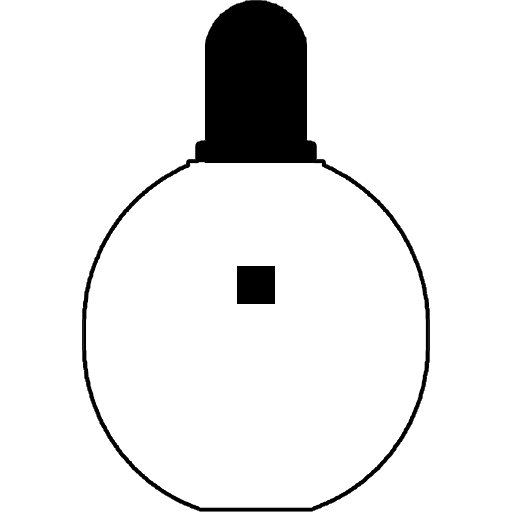
\includegraphics[width=1.15cm]{duo-logo-square-512.png}\\[1mm]
\end{minipage}

\vspace{1mm}
\hrule

\vspace{2.5mm}
\begin{multicols*}{2}


% --- INTERFACE ---
\tsection{Interface}
\begin{itemize}
    \item Mostly \textbf{SHORT} or \textbf{LONG} clicks
    \item A \textbf{SHORT} click is fast
    \item A \textbf{LONG} click requires 250ms
    \item Rare to \textbf{HOLD} the button
    \item Designed to reduce waiting around
\end{itemize}
\vspace{6pt}

% --- POWER FEATURES ---
\tsection{Primary Control}
\begin{itemize}
    \item \textbf{SHORT} click from OFF: Turn ON
    \item \textbf{LONG} click from OFF: Toggle Conjure
    \item \textbf{LONG} click from ON: Turn OFF
    \item \textbf{HOLD} from ON (past OFF): Menus
    \item 5x \textbf{SHORT} from OFF: Light Lock
    \item \textbf{HOLD} 10s: Force Sleep / Panic Exit
\end{itemize}
\vspace{6pt}

% --- MENUS & ENTRY ---
\msection{white}{https://stoneorbits.github.io/VortexEngine/menus.html}{Menus}
\desc{Edit mode or device settings}
\vspace{-1mm}
\begin{itemize}
    \item Same on all Vortex Devices
    \item In order of usefulness!
    \item Affect current mode:
    \begin{itemize}
	\item \led{whiteled} Randomizer
	\item \led{cyan} Mode Sharing
	\item \led{green} Color Select
	\item \led{blue} Pattern Select
    \end{itemize}
    \item Affect entire device:
    \begin{itemize}
	\item \led{yellow} Global Brightness
	\item \led{red} Factory Reset
    \end{itemize}
    \item Quick exit: go in random then exit
\end{itemize}
\vspace{8pt}

% --- LED SELECTION ---
\msection{purple}{https://stoneorbits.github.io/VortexEngine/led_selection.html}{LED Selection}

\begin{tikzpicture}[scale=0.6,baseline=0ex]
  % Example: two LEDs, one selected (highlighted), one not
  \draw[fill=purple,draw=white,thick] (0,0.25) circle (0.23);
  \draw[fill=grayslot,draw=white,thick] (0.52,0.25) circle (0.23);
\end{tikzpicture}
\desc{Pick target LED}
\begin{itemize}
  \item Some menus require LED selection
  \item Choose the affeced LED(s)
  \item \textbf{SHORT}: Cycle: tip, top, or both
  \item \textbf{LONG}: Confirm selection
\end{itemize}
\vspace{7pt}

% --- RANDOMIZER ---
\msection{whiteled}{https://stoneorbits.github.io/VortexEngine/randomizer_menu.html}{Randomizer}

\begin{tikzpicture}[scale=0.6, baseline=0ex]
  \filldraw[white,thick] (0,0) rectangle (0.5,0.5);
  \foreach \i/\j in {0.1/0.1, 0.4/0.4, 0.4/0.1, 0.1/0.4, 0.25/0.25}
    \fill[black] (\i,\j) circle (0.055);
\end{tikzpicture}
\desc{Roll new modes}
\begin{itemize}
    \item \led{purple}\led{gray} Select LED first
    \item \textbf{SHORT}: randomize new mode
    \item \textbf{LONG}: save \& exit
    \item \textbf{SHORT} 3x: Enable auto random
\end{itemize}
\vspace{8pt}

% --- MODE SHARING ---
\msection{cyan}{https://stoneorbits.github.io/VortexEngine/mode_sharing_menu.html}{Mode Sharing}

\begin{tikzpicture}[scale=0.33,baseline=-0.7ex]
  % Outer arc
  \draw[thick,cyan] (0.54,0.48) arc[start angle=50,end angle=-50,radius=0.8];
  % Middle arc
  \draw[thick,cyan] (0.36,0.3) arc[start angle=50,end angle=-50,radius=0.5];
  % Inner arc
  \draw[thick,cyan] (0.18,0.14) arc[start angle=50,end angle=-50,radius=0.22];
  % Dot (center)
  \fill[cyan] (0.02,-0.02) circle (0.07);
\end{tikzpicture}
\desc{Wirelessly share}
\begin{itemize}
    \item \textbf{SHORT} to cycle options
    \begin{itemize}
	\item \led{teal} Modern: \textbf{HOLD} to send
	\item \led{dimwhite} Legacy: \textbf{LONG} to send
	\item \led{red} Exit: \textbf{LONG} to leave
    \end{itemize}
\end{itemize}
\vspace{10pt}

% --- COLOR SELECT ---
\msection{green}{https://stoneorbits.github.io/VortexEngine/color_select_menu.html}{Color Select}

\begin{tikzpicture}[scale=0.8, baseline={([yshift=-.6ex]current bounding box.center)}]
  % Five colored circles representing a colorset
  \foreach \x/\c in {0/red, 1/green, 2/blue, 3/yellow, 4/purple} {
    \draw[fill=\c,draw=white,thick] (\x*0.25,0) circle (0.10);
  }
  % Optional: Add one "empty" slot (gray)
  \draw[fill=grayslot,draw=white,thick] (5*0.25,0) circle (0.10);
\end{tikzpicture}
\desc{Edit mode colors}
\begin{itemize}
    \item \led{purple}\led{gray} Select LED first
    \item Pick slot:
    \begin{itemize}
        \item Existing = edit, empty = add
        \item exit = shows colors + red on top
        \item HOLD on slot: delete
    \end{itemize}
    \item For slot:
    \begin{itemize}
        \item \textbf{Pick hue quadrant:}
	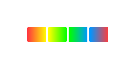
\begin{tikzpicture}[scale=0.64,baseline]
	  \shade[left color=red,right color=yellow]    (0*0.41,0) rectangle ++(0.36,0.28);
	  \shade[left color=yellow,right color=green]  (1*0.41,0) rectangle ++(0.36,0.28);
	  \shade[left color=green,right color=blue]    (2*0.41,0) rectangle ++(0.36,0.28);
	  \shade[left color=blue,right color=red]      (3*0.41,0) rectangle ++(0.36,0.28);
	\end{tikzpicture}
        \item \textbf{Pick fine hue:}
	
\begin{tikzpicture}[scale=0.64,baseline]
	  \fill[fill=blue!80!cyan]    (0*0.41,0) rectangle ++(0.36,0.28);
	  \fill[fill=blue]            (1*0.41,0) rectangle ++(0.36,0.28);
	  \fill[fill=blue!60!purple]  (2*0.41,0) rectangle ++(0.36,0.28);
	  \fill[fill=purple]          (3*0.41,0) rectangle ++(0.36,0.28);
	\end{tikzpicture}
        \item \textbf{Adjust saturation:}
	
\begin{tikzpicture}[scale=0.59,baseline]
	  \foreach \i in {0,...,3}
	    \fill[fill=blue!\the\numexpr30+23*\i\relax!white] (\i*0.38,0) rectangle ++(0.33,0.28);
	\end{tikzpicture}
        \item \textbf{Adjust brightness:}
	
\begin{tikzpicture}[scale=0.59,baseline]
	  \foreach \i in {0,...,3}
	    \fill[fill=blue!\the\numexpr40+18*\i\relax!black] (\i*0.38,0) rectangle ++(0.33,0.28);
	\end{tikzpicture}
        \item Returns to slot select
        \item Repeat or exit
    \end{itemize}
\end{itemize}
\vspace{9pt}

% --- PATTERN SELECT ---
\msection{blue}{https://stoneorbits.github.io/VortexEngine/pattern_select_menu.html}{Pattern Select}
\begin{tikzpicture}[scale=1.35,baseline]
  % Dot
  \draw[white,thick] (0,0.14) -- (0.05,0.14);
  \draw[white,thick] (0,0.12) -- (0.05,0.12);
  \draw[white,thick] (0,0.10) -- (0.05,0.10);
  \draw[white,thick] (0,0.08) -- (0.05,0.08);
  \draw[white,thick] (0,0.06) -- (0.05,0.06);
  % Dash
  \draw[white,thick] (0.10,0.14) -- (0.25,0.14);
  \draw[white,thick] (0.10,0.12) -- (0.25,0.12);
  \draw[white,thick] (0.10,0.10) -- (0.25,0.10);
  \draw[white,thick] (0.10,0.08) -- (0.25,0.08);
  \draw[white,thick] (0.10,0.06) -- (0.25,0.06);
  % Dot
  \draw[white,thick] (0.30,0.14) -- (0.35,0.14);
  \draw[white,thick] (0.30,0.12) -- (0.35,0.12);
  \draw[white,thick] (0.30,0.10) -- (0.35,0.10);
  \draw[white,thick] (0.30,0.08) -- (0.35,0.08);
  \draw[white,thick] (0.30,0.06) -- (0.35,0.06);
  % Dash
  \draw[white,thick] (0.40,0.14) -- (0.55,0.14);
  \draw[white,thick] (0.40,0.12) -- (0.55,0.12);
  \draw[white,thick] (0.40,0.10) -- (0.55,0.10);
  \draw[white,thick] (0.40,0.08) -- (0.55,0.08);
  \draw[white,thick] (0.40,0.06) -- (0.55,0.06);
\end{tikzpicture}
\desc{Edit mode pattern}
\begin{itemize}
    \item \led{purple}\led{gray} Select LED first
    \item \textbf{SHORT}: next pattern
    \item \textbf{LONG}: confirm/exit
\end{itemize}
\vspace{8pt}

% --- BRIGHTNESS ---
\msection{yellow}{https://stoneorbits.github.io/VortexEngine/global_brightness_menu.html}{Brightness}

\begin{tikzpicture}[scale=0.43,baseline=-0.2ex]
  \foreach \i in {1,2,3,4,5}
    \fill[yellow!85!white] (\i*0.23,0) rectangle ++(0.14,0.1*\i+0.05);
\end{tikzpicture}
\desc{Adjust brightness}
\begin{itemize}
    \item \textbf{SHORT}: Pick Brightness
    \item \textbf{LONG}: Save \& exit
\end{itemize}
\vspace{9pt}

% --- RESET ---
\msection{red}{https://stoneorbits.github.io/VortexEngine/factory_reset_menu.html}{Factory Reset}

\begin{tikzpicture}[scale=0.62,baseline=0ex]
  \draw[fill=red] (0,0) -- (0.3,0.52) -- (-0.3,0.52) -- cycle;
  \node[white] at (0,0.28) {\scriptsize\bfseries!};
\end{tikzpicture}
\desc{Reset device}
\begin{itemize}
    \item \textbf{SHORT}: Pick cancel or reset
    \begin{itemize}
	\item Cancel: Exit factory reset
	\item Reset: HOLD until solid white
    \end{itemize}
\end{itemize}
\vspace{8pt}

% --- Web Tools ---
\tsection{Web Tools}
\desc{Explore and share online}
\begin{itemize}
    \item Click \textbf{titles} in this document for Wiki!
    \item \href{https://lightshow.lol}{\texttt{lightshow.lol}} -- Build Modes
    \item \href{https://vortex.community}{\texttt{vortex.community}} -- Share Modes
    \item Find our discord on the \href{https://stoneorbits.github.io/VortexEngine/support.html}{\texttt{Wiki!}}
\end{itemize}

\end{multicols*}
\end{document}

